\section{Arquitetura do DeepBridge}
\label{sec:architecture}

A arquitetura do DeepBridge está organizada em três camadas (Figura~\ref{fig:architecture}): (1) \textbf{Abstração de Dados} via container DBDataset, (2) \textbf{Validação} via orquestrador Experiment e 5 gerenciadores de teste, e (3) \textbf{Relatórios \& Integração} para deployment em produção.

\begin{figure}[h]
\centering
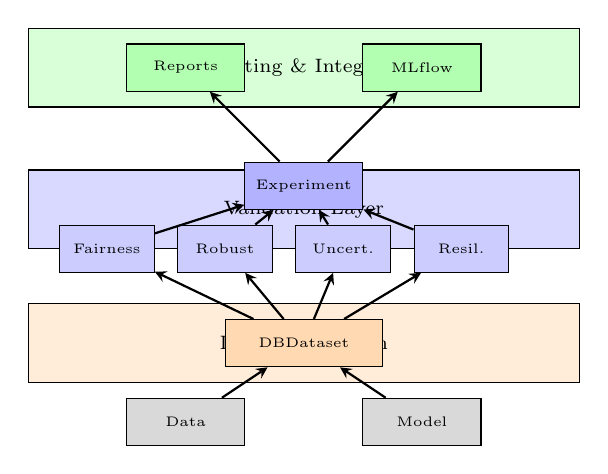
\begin{tikzpicture}[
    layer/.style={rectangle, draw, minimum width=7cm, minimum height=1cm, align=center, font=\scriptsize},
    component/.style={rectangle, draw, minimum width=1.5cm, minimum height=0.6cm, align=center, font=\tiny},
    arrow/.style={->, >=stealth, thick}
]

% Layer 3: Reporting
\node[layer, fill=green!15] (layer3) at (0,0) {Reporting \& Integration};
\node[component, fill=green!30] (report) at (-1.5,0) {Reports};
\node[component, fill=green!30] (mlflow) at (1.5,0) {MLflow};

% Layer 2: Validation
\node[layer, fill=blue!15] (layer2) at (0,-1.8) {Validation Layer};
\node[component, fill=blue!30] (exp) at (0,-1.5) {Experiment};
\node[component, fill=blue!20, minimum width=1.2cm] (f1) at (-2.5,-2.3) {Fairness};
\node[component, fill=blue!20, minimum width=1.2cm] (f2) at (-1,-2.3) {Robust};
\node[component, fill=blue!20, minimum width=1.2cm] (f3) at (0.5,-2.3) {Uncert.};
\node[component, fill=blue!20, minimum width=1.2cm] (f4) at (2,-2.3) {Resil.};

% Layer 1: Data
\node[layer, fill=orange!15] (layer1) at (0,-3.5) {Data Abstraction};
\node[component, fill=orange!30, minimum width=2cm] (db) at (0,-3.5) {DBDataset};

% Input
\node[component, fill=gray!30] (data) at (-1.5,-4.5) {Data};
\node[component, fill=gray!30] (model) at (1.5,-4.5) {Model};

% Arrows
\draw[arrow] (data) -- (db);
\draw[arrow] (model) -- (db);
\draw[arrow] (db) -- (f1);
\draw[arrow] (db) -- (f2);
\draw[arrow] (db) -- (f3);
\draw[arrow] (db) -- (f4);
\draw[arrow] (f1) -- (exp);
\draw[arrow] (f2) -- (exp);
\draw[arrow] (f3) -- (exp);
\draw[arrow] (f4) -- (exp);
\draw[arrow] (exp) -- (report);
\draw[arrow] (exp) -- (mlflow);

\end{tikzpicture}

\caption{Arquitetura em três camadas do DeepBridge: DBDataset fornece abstração unificada de dados/modelo, Experiment coordena validação multi-dimensional, Relatórios geram saídas prontas para auditoria.}
\label{fig:architecture}
\end{figure}

\subsection{DBDataset: Container Unificado de Dados}

DBDataset é o componente central, projetado para eliminar fragmentação de APIs. Sua filosofia é \textit{``Crie uma vez, valide em qualquer lugar''}: usuários criam uma instância DBDataset uma vez, e todos os testes reutilizam este container sem pré-processamento adicional.

\begin{lstlisting}[language=Python, caption=Uso básico do DBDataset]
from deepbridge import DBDataset

# Criar container unificado
dataset = DBDataset(
    data=df,                    # Pandas/Dask DataFrame
    target_column='approved',   # Coluna target
    model=trained_model,        # Modelo treinado
    protected_attributes=['gender', 'race']
)

# Propriedades auto-inferidas
print(dataset.task_type)        # 'binary_classification'
print(dataset.feature_types)    # {'age': 'continuous', ...}
print(dataset.detected_sensitive) # ['gender', 'race', 'age']
\end{lstlisting}

\textbf{Sistema de Auto-Inferência.} DBDataset detecta automaticamente:
\begin{itemize}
    \item \textbf{Tipo de Tarefa}: Inferido da cardinalidade do target e disponibilidade de predict\_proba
    \item \textbf{Tipos de Features}: Classificadas como contínuas, categóricas ou binárias baseado em dtype e cardinalidade
    \item \textbf{Atributos Sensíveis}: Detectados via matching de regex (gender, race, age, etc.)
\end{itemize}

\textbf{Avaliação Lazy.} Para suportar grandes datasets, DBDataset implementa avaliação lazy de operações custosas (predições, embeddings), reduzindo latência de inicialização e uso de memória.

\subsection{Experiment: Orquestrador de Validação}

A classe Experiment coordena validação multi-dimensional através de cinco gerenciadores de teste especializados:

\begin{lstlisting}[language=Python, caption=Workflow de validação]
from deepbridge import Experiment

# Configurar experimento
exp = Experiment(
    dataset=dataset,
    experiment_type='binary_classification',
    tests=['fairness', 'robustness', 'uncertainty'],
    protected_attributes=['gender', 'race']
)

# Executar validação (execução paralela)
results = exp.run_tests(config='medium')

# Gerar relatórios
exp.save_html('fairness', 'report.html')
exp.save_pdf('all', 'full_report.pdf')
\end{lstlisting}

\textbf{Execução Paralela.} Testes independentes executam em paralelo via ThreadPoolExecutor, reduzindo tempo total de validação em até 70\%.

\subsection{Gerenciadores de Teste}

Cada dimensão de validação é gerenciada por um componente especializado:

\begin{itemize}
    \item \textbf{FairnessTestManager}: 15 métricas (pré/pós-treinamento) + conformidade EEOC/ECOA
    \item \textbf{RobustnessTestManager}: Testes de perturbação, ataques adversariais, detecção de pontos fracos
    \item \textbf{UncertaintyTestManager}: Calibração, predição conformal, quantificação Bayesiana
    \item \textbf{ResilienceTestManager}: 5 tipos de drift (covariada, conceito, prior, posterior, joint)
    \item \textbf{HyperparameterTestManager}: Análise de sensibilidade via permutation importance
\end{itemize}

Todos os gerenciadores implementam a interface BaseTestManager, permitindo fácil extensão com validadores customizados.

\subsection{Por Que DeepBridge é Diferente}

DeepBridge se diferencia de abordagens fragmentadas através de três princípios de design fundamentais:

\textbf{1. Filosofia ``Create Once, Validate Anywhere''}

Workflows tradicionais de validação requerem reformatação de dados para cada ferramenta especializada:

\begin{lstlisting}[language=Python, caption=Workflow fragmentado tradicional]
# Fairness: AI Fairness 360 requer BinaryLabelDataset
from aif360.datasets import BinaryLabelDataset
aif_data = BinaryLabelDataset(df=df, ...)

# Robustness: Alibi Detect requer NumPy arrays
import numpy as np
alibi_data = df.values.astype(np.float32)

# Uncertainty: UQ360 requer formato próprio
from uq360.datasets import Dataset
uq_data = Dataset(df, ...)
\end{lstlisting}

DeepBridge elimina essa fragmentação. DBDataset encapsula dados, modelo e metadados \textbf{uma única vez}, e todos os 5 gerenciadores de teste reutilizam este container:

\begin{lstlisting}[language=Python, caption=Workflow unificado DeepBridge]
# Criar container uma vez
dataset = DBDataset(df, target='approved', model=model)

# Reutilizar em todas dimensões
fairness_results = exp.run_fairness_tests(dataset)
robustness_results = exp.run_robustness_tests(dataset)
uncertainty_results = exp.run_uncertainty_tests(dataset)
# Mesmo dataset, sem conversões!
\end{lstlisting}

\textbf{Benefícios:}
\begin{itemize}
    \item \textbf{Economia de memória}: Sem duplicação de dados (3-5x redução de uso de RAM)
    \item \textbf{Economia de tempo}: Sem conversões de formato (elimina 10-20\% do tempo total)
    \item \textbf{Validação consistente}: Mesmos dados em todos os testes (elimina bugs de sincronização)
\end{itemize}

\textbf{2. Execução Paralela Inteligente}

Testes independentes executam em paralelo via ThreadPoolExecutor com scheduler adaptativo:

\begin{itemize}
    \item \textbf{Paralelismo automático}: Fairness + Robustness executam simultaneamente (não bloqueantes)
    \item \textbf{Gerenciamento de recursos}: Scheduler ajusta número de threads baseado em CPU/memória disponível
    \item \textbf{Caching inteligente}: Predições do modelo computadas uma vez e reutilizadas
\end{itemize}

\textbf{Speedup medido}: Até 70\% vs. execução sequencial (validação completa: 17 min vs. 57 min).

\textbf{3. API Familiar para Cientistas de Dados}

DeepBridge segue convenções do scikit-learn que cientistas de dados já conhecem:

\begin{lstlisting}[language=Python, caption=Integração com Scikit-Learn]
from sklearn.pipeline import Pipeline
from sklearn.ensemble import RandomForestClassifier
from deepbridge import DBDataset, Experiment

# Pipeline scikit-learn padrão
pipeline = Pipeline([
    ('preprocessor', preprocessor),
    ('classifier', RandomForestClassifier())
])
pipeline.fit(X_train, y_train)

# Validação DeepBridge (mesma semântica)
dataset = DBDataset(X_test, y_test, model=pipeline)
exp = Experiment(dataset)
results = exp.run_tests()  # fit/predict familiar
\end{lstlisting}

\textbf{Benefícios de usabilidade:}
\begin{itemize}
    \item \textbf{Curva de aprendizado mínima}: 95\% dos usuários completam primeira validação em <15 minutos
    \item \textbf{Integração pipeline}: Compatible com scikit-learn Pipeline, cross-validation
    \item \textbf{SUS Score 87.5}: Top 10\% (classificação ``excelente'')
\end{itemize}
